%%%%%%%%%%%%%%%%%%%%%%%%%%%%%%%%%%%%%%%%%%%%%%%%%%%%%%%%%%%%%%%%%%%%
%%
%%                     Introdução
%%
%%%%%%%%%%%%%%%%%%%%%%%%%%%%%%%%%%%%%%%%%%%%%%%%%%%%%%%%%%%%%%%%%%%%


\begin{frame}{Introdução}

    \begin{figure}[!ht]
        \centering % para centralizar a figur
          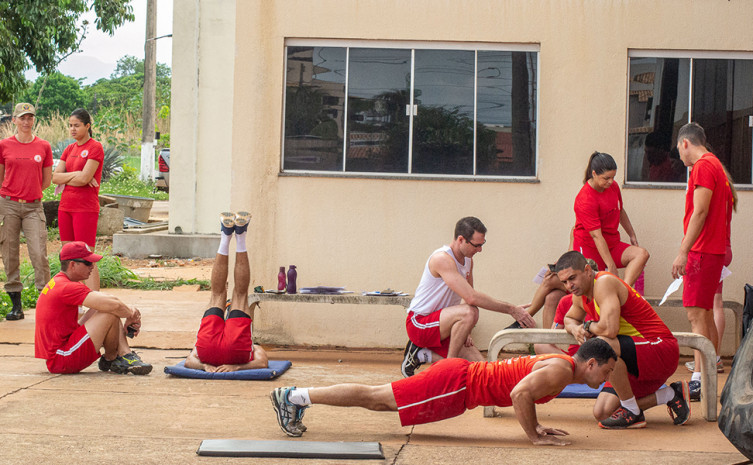
\includegraphics[scale=0.5]{img/intro/taf.jpeg}
         \caption{Teste de Aptidão Física - (TAF)}
    \end{figure}

\end{frame}


\begin{frame}{Introdução}

    \begin{figure}[!ht]
        \centering % para centralizar a figur
          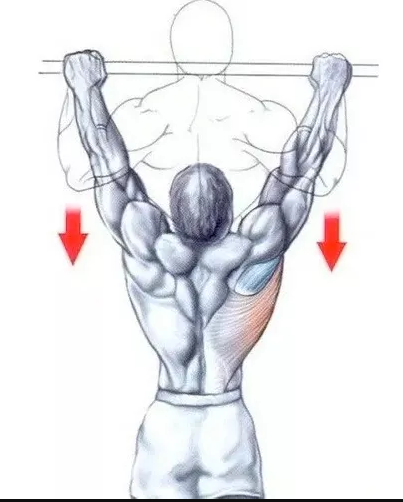
\includegraphics[scale=0.35]{img/intro/barra_fixa.png}
         \caption{Barra Fixa}
    \end{figure}

\end{frame}


%%%%%%%%%%%%%%%%%%%%%%%%%%%%%%%%%%%%%%%%%%%%%%%%%%%%%%%%%%%%%%%%%%%%
%%
%%                     Justificativa
%%
%%%%%%%%%%%%%%%%%%%%%%%%%%%%%%%%%%%%%%%%%%%%%%%%%%%%%%%%%%%%%%%%%%%%


\begin{frame}{Justificativa}
    \begin{block}{ Potencial para aumentar a confiabilidade e justiça do processo seletivo}
        \begin{itemize}
            \item  Minimiza os efeitos da fadiga de decisão dos avaliadores;
            \item  Minimiza a subjetividade na avaliação do exercício de barra fixa;
        \end{itemize}
    \end{block}
\end{frame}


\begin{frame}{Justificativa}
    \begin{block}{Contribuição para a evolução da maturidade da consciência corporal do indivíduo.}
        \begin{itemize}
            \item A percepção durante o exercício é essencial para o aprimoramento do movimento.
            \item Gera a tomada de consciência do corpo em relação ao movimento da barra fixa.
        \end{itemize}
    \end{block}
\end{frame}


\begin{frame}{Justificativa}
    \begin{block}{Contribuição para o treinamento no TAF}
        \begin{itemize}
            \item Fornece o feedback sobre a execução correta do movimento.
        \end{itemize}
    \end{block}
\end{frame}




%%%%%%%%%%%%%%%%%%%%%%%%%%%%%%%%%%%%%%%%%%%%%%%%%%%%%%%%%%%%%%%%%%%%
%%
%%                     Objetivos
%%
%%%%%%%%%%%%%%%%%%%%%%%%%%%%%%%%%%%%%%%%%%%%%%%%%%%%%%%%%%%%%%%%%%%%

\begin{frame}{Objetivos}
    \begin{block}{Objetivo Geral}
    Este trabalho tem como objetivo projetar e desenvolver uma ferramenta de visão computacional para análise do movimento de barra fixa associada ao TAF.
    \end{block}

\end{frame}



\begin{frame}{Objetivos}
   
    \begin{block}{Objetivos Específicos}
        \begin{itemize}
            \item Desenvolver uma ferramenta de visão computacional (em nível de prova de conceito) que analise o movimento de barra fixa.
                \begin{itemize}
                    \item Identificar a corretude do movimento de barra fixa.
                    \item Definir um procedimento para estabelecer a corretude do movimento de barra fixa, tendo como parâmetros alguns editais de concursos públicos da esfera militar
                    \item Analisar o movimento de barra fixa de modo a auxiliar na formação da consciência corporal do indivíduo por meio de feedback.
                \end{itemize}
            \item Usar a visão computacional para validar a corretude do movimento de barra fixa, tendo como parâmetros alguns editais de concursos públicos da esfera militar.
        \end{itemize}
    \end{block}

\end{frame}




